\pagestyle{empty}
\nopagecolor
\begin{flushleft}

\includegraphics[width=6cm]{Packt_logo-grey}\\
\url{www.packt.com}

\vspace{0.2 cm}

Subscribe to our online digital library for full access to over 7,000 books and videos, as well as industry leading tools to help you plan your personal development and advance your career. For more information, please visit our website.

\section*{Why subscribe?}
\begin{itemize}[nosep]
    \item Spend less time learning and more time coding with practical eBooks and Videos from over 4,000 industry professionals
    \item Improve your learning with Skill Plans built especially for you
    \item Get a free eBook or video every month
    \item Fully searchable for easy access to vital information
    \item Copy and paste, print, and bookmark content
\end{itemize}

\vspace{0.2 cm}

Did you know that Packt offers eBook versions of every book published, with PDF and ePub files available? You can upgrade to the eBook version at packt.com and as a print book customer, you are entitled to a discount on the eBook copy. Get in touch with us at \href{mailto:customercare@packtpub.com}{customercare@packtpub.com} for more details.

\vspace{0.2 cm}

At \url{www.packt.com}, you can also read a collection of free technical articles, sign up for a range of free
\newpage
\section*{Other Books You Might Enjoy}
If you enjoyed this book, you may be interested in these other books by Packt:\\

\vspace{0.2 cm}

%\begin{center}
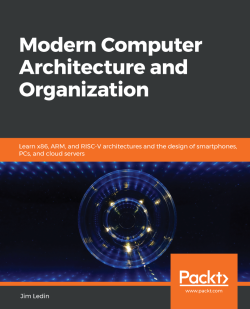
\includegraphics[width=3cm]{9781838984397}\\
%\end{center}

\vspace{0.2 cm}

{\fontfamily{ppl}\AlegreyaSansMedium Modern Computer Architecture and Organization}\\
\vspace{0.2 cm}
Jim Ledin\\
ISBN: 978-1-83898-439-7\\

\begin{itemize}[nosep]
    \item Get to grips with transistor technology and digital circuit principles
    \item Discover the functional elements of computer processors
    \item Understand pipelining and superscalar execution
    \item Work with floating-point data formats
    \item Understand the purpose and operation of the supervisor mode
    \item Implement a complete RISC-V processor in a low-cost FPGA
    \item Explore the techniques used in virtual machine implementation
    \item Write a quantum computing program and run it on a quantum computer
\end{itemize}

\vspace{0.3 cm}

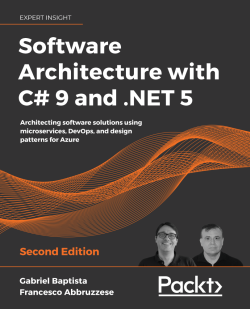
\includegraphics[width=3cm]{9781800566040}\\

\vspace{0.2 cm}

{\fontfamily{ppl}\AlegreyaSansMedium Software Architecture with C\# 9 and .NET 5 - Second Edition}\\

\vspace{0.2 cm}

Gabriel Baptista, Francesco Abbruzzese\\
ISBN: 978-1-80056-604-0\\

\begin{itemize}[nosep]
    \item Use different techniques to overcome real-world architectural challenges and solve design consideration issues
    \item Apply architectural approaches such as layered architecture, service-oriented architecture (SOA), and microservices
    \item Leverage tools such as containers, Docker, Kubernetes, and Blazor to manage microservices effectively
    \item Get up to speed with Azure tools and features for delivering global solutions
    \item Program and maintain Azure Functions using C\# 9 and its latest features
    \item Understand when it is best to use test-driven development (TDD) as an approach for software development
    \item Write automated functional test cases
    \item Get the best of DevOps principles to enable CI/CD environments
\end{itemize}

\section*{Packt is searching for authors like you}
If you're interested in becoming an author for Packt, please visit \url{authors.packtpub.com} and apply today. We have worked with thousands of developers and tech professionals, just like you, to help them share their insight with the global tech community. You can make a general application, apply for a specific hot topic that we are recruiting an author for, or submit your own idea.

\vspace{0.2 cm}

\section*{Share Your Thoughts}
Now you’ve finished \textbf {NameOfTheProduct}, we’d love to hear your thoughts! Scan the QR code below to go straight to the Amazon review page for this book and share your feedback.

\begin{center}

\includegraphics[width=3cm]{qr-code}\\
%\URL{https://packt.link/r/<ISBN10P>}
\small{https://packt.link/r/<ISBN10P>}
\end{center}

Your review is important to us and the tech community and will help us make sure we’re delivering excellent quality content.

\hl{Replace \textbf{NameOfTheProduct} with your title name.}
\newline
\hl{Replace the dummy QR Code image with your product QR code image.}
\newline
\hl{Replace \textit{ISBN10P} with the 10-digit \textit{ISBN-10P} from EPIC.}
\newline
\hl{This page should be added after the Front Matter.}

\clearpage

\end{flushleft}